\section{Описание}
{\bfseries Корпус документов.}

Так как стоит задача построения распределения слов в исходных текстах, необходимо устранить такие проблемы данных, как наличие знаков препинания и заглавных символов - выбросим все вхождения знаков препинания в текст и приведём его к нижнему регистру. Построим распределение слов в полученном обработанном тексте для каждого жанра, а затем выберем 10 наиболее встречающихся слов - получим следующую картину:


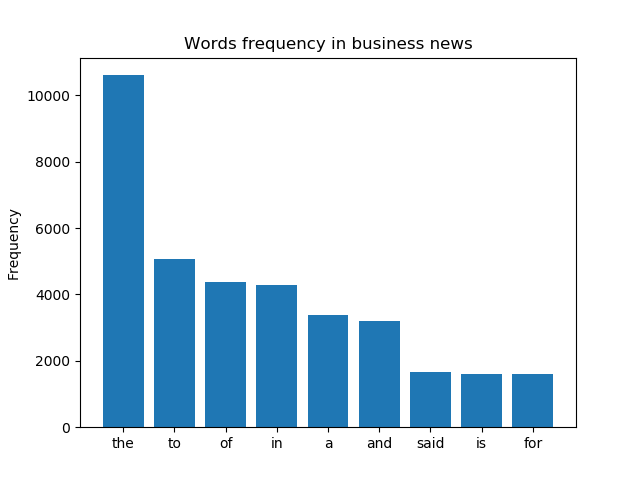
\includegraphics[width=0.5\linewidth]{src/business.png}
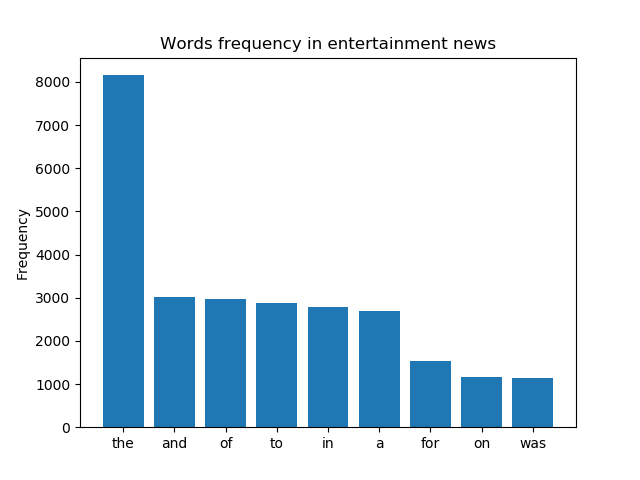
\includegraphics[width=0.5\linewidth]{src/entertainment.png}
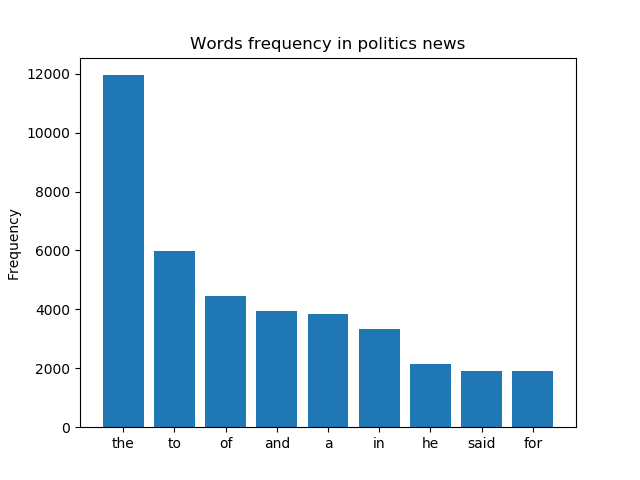
\includegraphics[width=0.5\linewidth]{src/politics.png}
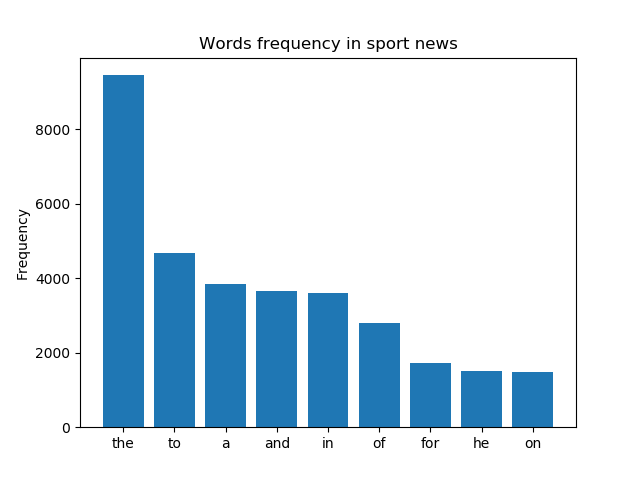
\includegraphics[width=0.5\linewidth]{src/sport.png}
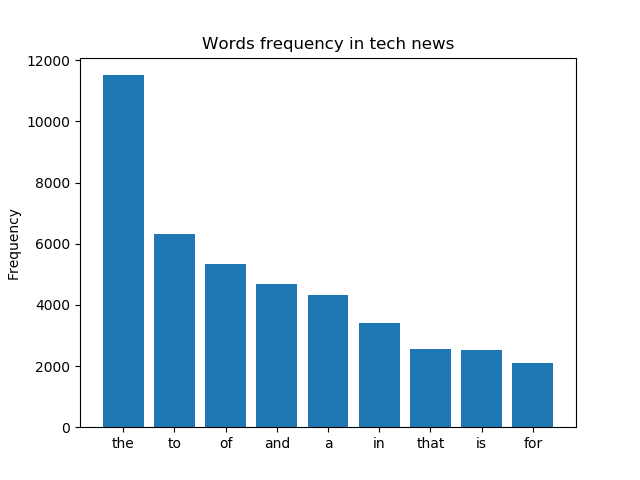
\includegraphics[width=0.5\linewidth]{src/tech.png}

Проанализировав полученные результаты, можно сделать вывод, что вне зависимости от жанра текста наиболее популярными словами будут короткие (3-4 буквы) слова-связки, а также слова, обозначающие косвенную/прямую прямую речь (said), что свойственно для текстов типа новостей.

\lstset{  
    caption=\lstname
}
\lstinputlisting[language=Python]{src/bbc.py}

{\bfseries Данные котировок акций.}

Исходные данные о котировках акций за некоторый промежуток времени представлены в виде отдельных файлов - каждый файл характеризует конкретную акцию. Можно соединить все акции в один .csv файл, при этом общий размер увеличится. Если сделать предположение, что котировки одной акции не зависят от котировок других(а так в большинстве случаев и есть), то можно рассматривать каждый файл, как отдельный датасет.

При рассмотрении датасета выяснилось, что некоторые файлы пусты, эти акции необходимо удалить, так как они не несут никакой смысловой нагрузки.
\lstinputlisting[language=Python]{src/a.py}
Каждая акция содержит 7 признаков:
\begin{enumerate}
    \item Date - день котировки
    \item Open - цена на открытии биржи
    \item High - наибольшая цена за день
    \item Low - наименьшая цена за день
    \item Close - цена на закрытии биржи
    \item Volume - суммарное количество операций за день
    \item OpenInt(Open Interest) - сумма открытых позиций
\end{enumerate}

В случае акций, величина Open Interest всегда равна 0(имеет ненулевое значение для фьючерсов и других срочных контрактов), поэтому её стоит исключить из обработки данных. Volume - не слишком информативный признак, так как на предсказание цены акции влияет её история и экономическая ситуация, но никак не количество торгуемых акций, поэтому её так же можно исключить.

Построим распределение признаков акций, найдём среднее, дисперсию, медиану и некоторые квантили и изобразим наиболее "интересные" из них.
\lstinputlisting[language=Python]{src/statistics.py}
\lstinputlisting[language=Python]{src/stats.py}

Классический пример - акции Apple.

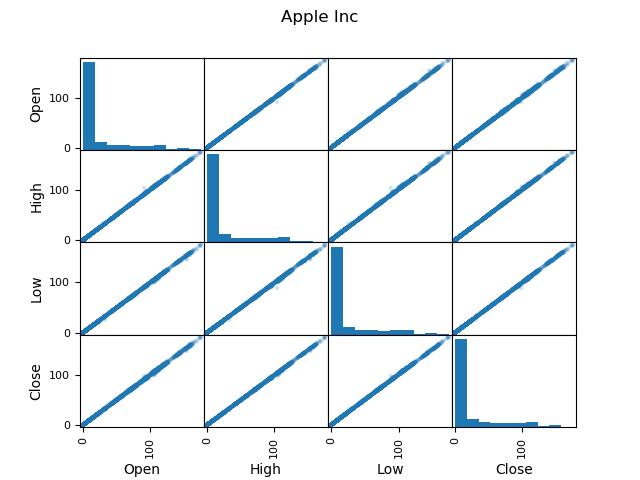
\includegraphics[width=0.5\linewidth]{src/aapl1.png}
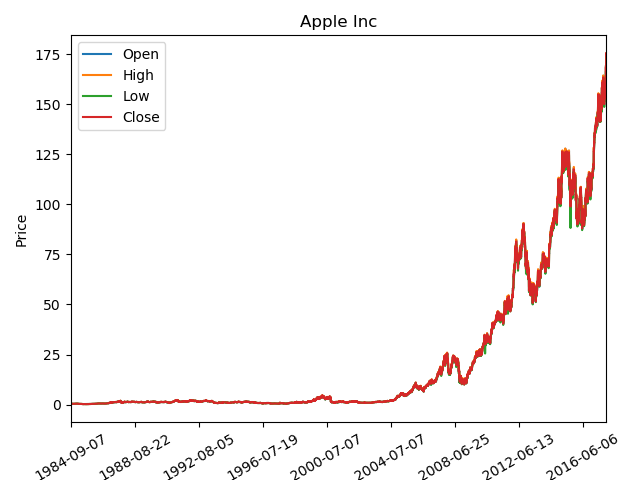
\includegraphics[width=0.5\linewidth]{src/aapl2.png}

Метод scatter\_matrix строит распределение признаков, а также зависимость одного признака от другого. Как видно из графика котировок, акция в среднем росла, что и отражено в виде прямой с углом наклона $\dfrac{\pi}{4}$.

Числовые характеристики:
\lstinputlisting{src/aapl.csv}

Более интересная картина наблюдается с акциями Eyegate Pharma:

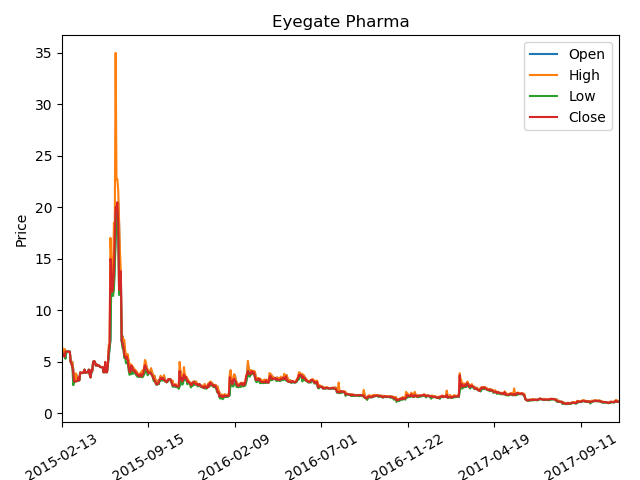
\includegraphics[width=0.5\linewidth]{src/eyeg1.png}
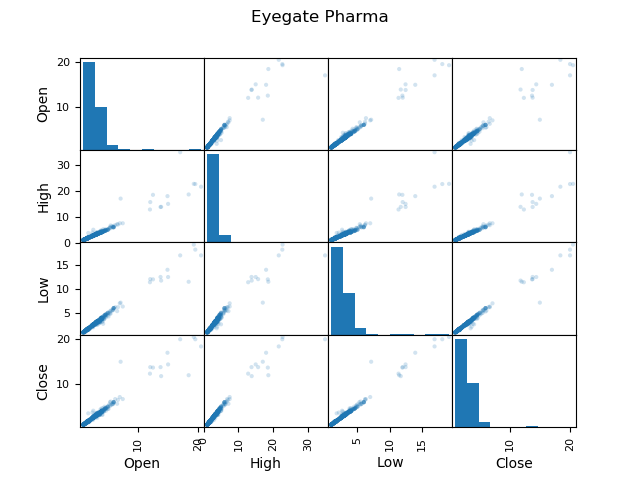
\includegraphics[width=0.5\linewidth]{src/eyeg2.png}

Характерный пик в стоимости акций отражается на зависимости одного признака от другого, а также в статистических характеристиках.
\lstinputlisting{src/eyeg.csv}

В данном датасете можно попробовать, например, предсказать цену акции на открытии торгов по данным, полученным за другой период, или максимальное падение акции за день в течение торгов. 